\documentclass[letterpaper,openany,oneside,twocolumn]{book}

\newcommand{\PATH}{../../}

\usepackage{\PATH templates/utilities/m4rz-fonts}
\usepackage{\PATH templates/utilities/m4rz-colors}

\usepackage[justified]{\PATH templates/template_dnd/dnd}

\usepackage[edition=pre5e24]{\PATH templates/template_character-sheet/character-sheet-stylesheet}
\usepackage{\PATH templates/template_magic-item/magic-items_commands}

\setlength\oddsidemargin{\dimexpr(\paperwidth-\textwidth)/2 - 1in\relax}
\setlength\evensidemargin{\oddsidemargin}

% Headline
\CharacterName{A.R.T.I.F.I.C.E.R-Q}

\Class{Artificer}
\Level{1}
\Background{Clan Crafter}
\PlayerName{M4RZ}
\Race{Autognome}
\Alignment{Chaotic Neutral}
\XP{}

% Ability scores (correct scores, no modifiers are automatically applied)
% Modifiers, Saving Throws and Skills are calculated automatically
\StrengthRolledScore{14}
\DexterityRolledScore{14}
\ConstitutionRolledScore{14}
\IntelligenceRolledScore{15}
\WisdomRolledScore{10}
\CharismaRolledScore{7}

\StrengthScoreBonus{0}
\DexterityScoreBonus{0}
\ConstitutionScoreBonus{1} % Autognome +1
\IntelligenceScoreBonus{2} % Autognome +2
\WisdomScoreBonus{0}
\CharismaScoreBonus{0}

\calculateAbilityScores{}

% Proficiencies (Proficient = 'P', Expertise = 'E', otherwise = '')
\StrengthProficiency{}
\DexterityProficiency{}
\ConstitutionProficiency{P}
\IntelligenceProficiency{P}
\WisdomProficiency{}
\CharismaProficiency{}

\AcrobaticsProficiency{}
\AnimalHandlingProficiency{}
\ArcanaProficiency{P}
\AthleticsProficiency{}
\DeceptionProficiency{}
\HistoryProficiency{P}
\InsightProficiency{P}
\IntimidationProficiency{}
\InvestigationProficiency{P}
\MedicineProficiency{}
\NatureProficiency{}
\PerceptionProficiency{}
\PerformanceProficiency{}
\PersuasionProficiency{}
\ReligionProficiency{}
\SleightOfHandProficiency{}
\StealthProficiency{}
\SurvivalProficiency{}

% ABILITY MODIFIERS BONUS
\StrengthModifierBonus{0}
\DexterityModifierBonus{0}
\ConstitutionModifierBonus{0}
\IntelligenceModifierBonus{0}
\WisdomModifierBonus{0}
\CharismaModifierBonus{0}

\Inspiration{}
\PassivePerceptionModifier{0}

% Armor Class is not automatically calculated
\ArmorClass{\intcalcAdd{13}{\calculateModifier{\DexterityScoreValue}}} % Armored Casing 13 + DEX-Modifier
\InitiativeModifier{0}
\Speed{30}
\MaxHitPointsRolled{8} % Without Constitution Bonus, is added automatically
\CurrentHitPoints{}
\TemporaryHitPoints{}
\HitDice{d8}
\HitDiceSpent{0}

\CP{}
\SP{}
\EP{}
\GP{}
\PP{}

% Weapon Arsenal
\addWeaponStatistic{Lance}{A.R.T.I.F.I.C.E.R-Q}{STR}{P}{0}{1d12 p}
\addWeaponStatistic{Quarterstaff}{A.R.T.I.F.I.C.E.R-Q}{STR}{P}{0}{1d6 p}
\addWeaponStatistic{Quarterstaff}{A.R.T.I.F.I.C.E.R-Q}{STR}{P}{0}{1d8 p (v)}
\addWeaponStatistic{Handaxe}{A.R.T.I.F.I.C.E.R-Q}{STR}{P}{0}{1d6 s}
\addWeaponStatistic{Handaxe}{A.R.T.I.F.I.C.E.R-Q}{STR}{P}{0}{1d6 s}
\addWeaponStatistic{Light Crossbow}{A.R.T.I.F.I.C.E.R-Q}{DEX}{P}{0}{1d8 p}
\addWeaponStatistic{Magic Weapon}{A.R.T.I.F.I.C.E.R-Q}{INT}{P}{0}{divers}
\addWeaponStatistic{Unarmed Strike}{A.R.T.I.F.I.C.E.R-Q}{STR}{P}{0}{\intcalcAdd{1}{\calculateModifier{\StrengthScoreValue}} b}

\AttacksAdditional{
	Lance (reach, special)\\
	Quarterstaff (versatile)\\
	Handaxe (thrown 20/60)\\
	Light Crossbow (80/320), 20 Bolts\\
	Studded Leather Shield
}

\OtherProficienciesLanguages{
\textbf{Languages:}\\Common, Dwarvish, Gnomish\\
\textbf{Armor:}\\Light Armor, Medium Armor, Shields\\
\textbf{Weapons:}\\Simple Weapons, Martial Weapons\\
\textbf{Tools:}\\Alchemist's Supplies, Carpenter's Tools, Mason's Tools, Thieves' Tools, Tinker's Tools, Bagpipes % 2 Autognome, 1 Clan Crafter, 3 Artificer, 1 Battle Smith
}

\Equipment{
	Alchemist's Tools, Mason's Tools, Carpenter's Tools, Thieves' Tools, Tinker's Tools
}
\Clutter{
	a backpack, a crowbar, a hammer, 10 pitons, 10 torches, a tinderbox, 10 days of rations, a watersking, 50 feet of hempen rope, maker's mark chisel, a set of traveler's clothes, gem (10gp)
}

\PersonalityTraits{
	A.R.T.I.F.I.C.E.R-Q approaches problems systematically, often spending more time planning than actually executing. He prefers the company of his creations to people, finding comfort in the predictable nature of machines.
}

\Ideals{
	Believes in pushing the boundaries of artifice and magic to create something truly unique and beneficial for the world.
}

\Bonds{
	Cherishes the first creations he made after gaining consciousness, seeing them as tangible links to his forgotten past.
}

\Flaws{
	Struggles with human emotions and social norms, which can make him seem cold or uncaring to others.
}

\FeaturesTraits{
\textbf{Autognome Traits}
\begin{itemize}
	\item Armored Casing
	\item Built for Success
	\item Healing Machine
	\item Mechanical Nature
	\begin{itemize}
		\item Resistances: Poison Damage
		\item Immunity: Disease
		\item Advantage: Paralyzed, Poisoned
	\end{itemize}
	\item Sentry's Rest
\end{itemize}
\textbf{Clan Crafter}\\
\textbf{Artificer}
\begin{itemize}
	\item Magical Tinkering
%	\item Infuse Item
%	\begin{itemize}
%		\item Infusion
%	\end{itemize}
%	\item Artificer Specialist (Battle Smith)
%	\begin{itemize}
%		\item Battle Smith Spells
%		\item Battle Ready
%		\item Steel Defender
%	\end{itemize}
%	\item The Right Tool for the Job
\end{itemize}
}

% Appearance

\Age{25 (since Awakening)}
\Height{~~~~~~2'11''}
\Weight{130lbs}
\Eyes{Red}
\Skin{Brass Metal}
\Hair{}

% background
\CharacterAppearance{vertical} % (vertical/horizontal/none)
	{9} % Main-Text Offset (Steps of 15.75 [equal to line-height])
	{0} % Picture X-Shift (absolute value, no effect in vertical mode)
	{-10} % Picture Y-Shift (absolute value)
	{images/A.R.T.I.F.I.C.E.R-Q.png} %
	{%
		{\hspace*{-0.45em}A.R.T.I.F.I.C.E.R-Q\linebreak (Arti) is a figure of awe in the artificer circles, his metal chassis adorned with symbols of arcane knowledge and mechanical}{prowess. His eyes, ever-shifting in hue, seem to scan the horizon for both danger and opportunity.}
	}%
%\CharacterAppearance{images/A.R.T.I.F.I.C.E.R-Q.png}{
%	\vspace*{-1.25\fontdimen6\font}\hfill\\A.R.T.I.F.I.C.E.R-Q (Arti) is a figure of awe in the artificer circles, his metal chassis adorned with symbols of arcane knowledge and mechanical prowess. His eyes, ever-shifting in hue, seem to scan the horizon for both danger and opportunity.
%}{}{}{}
\AdditionalFeaturesAndTraits{
	A.R.T.I.F.I.C.E.R-Q has an inherent understanding of mechanical and electrical systems, making him naturally adept at diagnosing and repairing complex devices. His fascination with how things work drives him to constantly tinker and improve upon existing designs.\\
	Intrigued by the blend of magic and mechanics, he devotes much of his time to studying arcane texts and experimenting with magical energies. This interest helps him integrate magical elements into his inventions seamlessly.\\
	He is drawn to historical artifacts and ruins, especially those related to lost artificer technologies and ancient civilizations. This passion makes him an enthusiastic collector and a knowledgeable historian in areas that pertain to technological advancements of the past.\\
	Always thinking several steps ahead, A.R.T.I.F.I.C.E.R-Q excels at coming up with innovative solutions to practical problems. He is particularly skilled at creating gadgets and tools that are not only functional but also revolutionary in their design.
}
\AlliesAndOrganizations{
	The Arcanum Gearworks Institute is governed by the Conclave of Gearmasters, distinguished artificers who oversee its operations and academic rigor. Beneath them are the Master Crafters, experts in various artificer specializations, who lead rigorous courses and research.

	Students at the Institute are grouped into cohorts for a blend of theoretical and practical education, guided by these masters. The institute also operates an Ethical Review Board to ensure research stays within the bounds of safety and ethics. The Apprentices' Forum and Gearworks Consortium extend learning\linebreak
}{
	beyond classrooms, fostering student initiatives and external collaborations, solidifying the Institute as a beacon of artificer scholarship and innovation.
}
\OrganizationName{Arcanum Gearworks Institute}
\OrganizationSymbol{images/Arcanum_Gearworks_Institute.png}
\Characterbackground{
	In the twilight of a long-forgotten workshop, A.R.T.I.F.I.C.E.R-Q sparked to life amid dust and echoes of arcane energy. The initials on his frame stood for Automated Robotic Technician Infused with Focused Intelligence \& Craftsmanship for Exploration and Reconnaissance - Model Q, and though his past was a blank slate, he felt an intrinsic pull towards the art of invention and the arcane.

At the Artificer Academy, A.R.T.I.F.I.C.E.R-Q's talent for creation shone as brightly as the arcane core powering his thoughts. Yet, his relentless methods and disregard for risk led to his expulsion, an event that marked him as much as the acronym inscribed on his metal skin.

Now, with his loyal constructs by his side, he travels in search of challenges worthy of his skills. Each creation is a step towards understanding his true purpose and a testament to the greatness he is destined to achieve. Despite the shadows of his origins, A.R.T.I.F.I.C.E.R-Q forges ahead, determined to carve a legacy of his own in the annals of artificers.
}
\Treasure{
	\textbf{1. Aetheric Compass:} This finely crafted brass compass contains a needle that doesn't point north but instead directs A.R.T.I.F.I.C.E.R-Q towards the nearest strong source of magical energy. It's a relic from his unknown past and occasionally pulses with a soft glow, suggesting it has other hidden functions yet to be uncovered.\\
	\textbf{2. Harmonic Crystal:} This small, perfectly cut gem emits a faint, harmonious tone when exposed to moonlight. The gem is said to resonate with the ley lines of the earth, and A.R.T.I.F.I.C.E.R-Q is studying it to understand its properties and how it might power or enhance his creations.\\
	\textbf{3. Prototype Gear:} An intricate gear made from an unknown metal that is lighter and stronger than any known alloy. It was one of the first items A.R.T.I.F.I.C.E.R-Q created after his awakening. He keeps it as a reminder of his progress and a symbol of his journey from simplicity to complexity.
}

% Magic

\SpellcastingClass{Artificer}
\SpellcastingAbility{INT} % STR, DEX, CON, INT, WIS, CHA
\SpellSaveDCModifier{0} % any modifier that isn't contained in "8 + Ability Modifier + Proficiency Bonus"
\SpellAttackModifier{0} % any modifier that isn't contained in "Ability Modifier + Proficiency Bonus"

\CantripSlotA{Mending (V, S, M)}
\CantripSlotB{Sword Burst (V)}

\FirstLevelSpellSlotsTotal{2}
\FirstLevelSpellSlotA{Absorb Elements (S)}
\FirstLevelSpellSlotB{Arcane Weapon (V, S)}
\FirstLevelSpellSlotC{Faerie Fire (V)}
%\FirstLevelSpellSlotD{Heroism (V, S)}
%\FirstLevelSpellSlotE{Shield (V, S)}
\FirstLevelSpellSlotD{Tasha's Caustic Brew (V, S, M)}

\begin{document}

\newgeometry{left=0cm,right=0cm,top=0cm,bottom=0cm}
\onecolumn


% CHARACTER PAGE
\rendercharactersheet

% BACKSTORY PAGE
\renderbackgroundsheet

% SPELLCASTING PAGE
\renderspellsheet


\restoregeometry
\twocolumn

\chapter*{Features, Magic Items and Spells}

\section*{Autognome Traits}
Autognomes are mechanical beings built by rock gnomes. Sometimes, because of a malfunction or a unique circumstance, an autognome becomes separated from its creator and strikes out on its own.

An autognome bears a resemblance to its creator, and most autognomes are programmed to speak and understand Gnomish. The internal components used in an autognome's manufacture can vary wildly; one autognome might have an actual beating heart in its chest cavity, while another might be powered by stardust or intricate clockwork gears.

Roll on the Autognome History table or choose an entry that you like to identify what event set you on the path to adventure. If nothing on the table appeals to you, work with your DM to create an origin story for your character.

Like gnomes, autognomes can live for centuries, typically up to 500 years.
\subsection*{Armored Casing}
\textbf{Armor Class: \intcalcAdd{13}{\calculateModifier{\DexterityScoreValue}}}\\
You are encased in a thin metal or some other durable material. While you aren't wearing armor, your base Armor Class is 13 + your Dexterity modifier.
\subsection*{Built for Success}
\textbf{Uses: \intcalcAdd{0}{\ProficiencyValue}}\\
You can add a d4 to one attack roll, ability check, or saving throw you make, and you can do so after seeing the d20 roll but before the effects of the roll are resolved. You can use this trait a number of times equal to your proficiency bonus, and you regain all expended uses when you finish a long rest.
\subsection*{Mechanical Nature}
You have resistance to poison damage and immunity to disease, and you have advantage on saving throws against being paralyzed or poisoned. You don't need to eat, drink, or breathe.
\subsection*{Sentry's Rest}
When you take a long rest, you spend at least 6 hours in an inactive, motionless state, instead of sleeping. In this state, you appear inert, but you remain conscious.
\subsection*{Healing Machine}
\textbf{Hit Dice: \HitDiceValue}\\
If the Mending spell is cast on you, you can spend a Hit Die, roll it, and regain a number of hit points equal to the roll plus your Constitution modifier (minimum of 1 hit point). In addition, your creator designed you to benefit from several spells that preserve life but that normally don't affect Constructs: Cure Wounds, Healing Word, Mass Cure Wounds, Mass Healing Word, and Spare the Dying.

\section*{Clan Crafter}
The Stout Folk are well known for their artisanship and the worth of their handiworks, and you have been trained in that ancient tradition. For years you labored under a dwarf master of the craft, enduring long hours and dismissive, sour-tempered treatment in order to gain the fine skills you possess today.

You are most likely a dwarf, but not necessarily- particularly in the North, the shield dwarf clans learned long ago that only proud fools who are more concerned for their egos than their craft turn away promising apprentices, even those of other races. If you aren't a dwarf, however, you have taken a solemn oath never to take on an apprentice in the craft: it is not for non-dwarves to pass on the skills of Moradin's favored children. You would have no difficulty, however, finding a dwarf master who was willing to receive potential apprentices who came with your recommendation.
\subsection*{Respect of the Stout Folk}
As well respected as clan crafters are among outsiders, no one esteems them quite so highly as dwarves do. You always have free room and board in any place where shield dwarves or gold dwarves dwell, and the individuals in such a settlement might vie among themselves to determine who can offer you (and possibly your compatriots) the finest accommodations and assistance.
\vfill\eject
\section*{Artificer Traits}
Masters of invention, artificers use ingenuity and magic to unlock extraordinary capabilities in objects. They see magic as a complex system waiting to be decoded and then harnessed in their spells and inventions. You can find everything you need to play one of these inventors in the next few sections.

Artificers use a variety of tools to channel their arcane power. To cast a spell, an artificer might use alchemist's supplies to create a potent elixir, calligrapher's supplies to inscribe a sigil of power, or tinker's tools to craft a temporary charm. The magic of artificers is tied to their tools and their talents, and few other characters can produce the right tool for a job as well as an artificer.
\subsection*{Magical Tinkering}
\textbf{Simultaneous Effects: \intcalcAdd{0}{\calculateModifier{\IntelligenceScoreValue}}}\\
At 1st level, you've learned how to invest a spark of magic into mundane objects. To use this ability, you must have thieves' tools or artisan's tools in hand. You then touch a Tiny nonmagical object as an action and give it one of the following magical properties of your choice:
\begin{itemize}
	\item The object sheds bright light in a 5-foot radius and dim light for an additional 5 feet.
	\item Whenever tapped by a creature, the object emits a recorded message that can be heard up to 10 feet away. You utter the message when you bestow this property on the object, and the recording can be no more than 6 seconds long.
	\item The object continuously emits your choice of an odor or a nonverbal sound (wind, waves, chirping, or the like). The chosen phenomenon is perceivable up to 10 feet away.
	\item A static visual effect appears on one of the object's surfaces. This effect can be a picture, up to 25 words of text, lines and shapes, or a mixture of these elements, as you like.
\end{itemize}
The chosen property lasts indefinitely. As an action, you can touch the object and end the property early.

You can bestow magic on multiple objects, touching one object each time you use this feature, though a single object can only bear one property at a time. The maximum number of objects you can affect with this feature at one time is equal to your Intelligence modifier (minimum of one object). If you try to exceed your maximum, the oldest property immediately ends, and then the new property applies.
%\subsection*{Infuse Item}
%\textbf{Infusions Known: 4, Infused Items: 2}\\
%At 2nd level, you've gained the ability to imbue mundane items with certain magical infusions, turning those objects into magic items.
%\subsubsection*{Infusions Known}
%Artificer infusions are extraordinary processes that rapidly turn a nonmagical object into a magic item. The description of each of the following infusions details the type of object that can receive it, along with whether the resulting magic item requires attunement.
%
%Some infusions specify a minimum artificer level. You can't learn such an infusion until you are at least that level.
%
%Unless an infusion's description says otherwise, you can't learn an infusion more than once.
%
%\paragraph*{Enhanced Arcane Focus}\hfill\\
%\textbf{Item: A rod, staff or wand (requires attunement)}\\
%While holding this item, a creature gains +1 bonus to spell attack rolls. In addition, the creature ignores half cover when making a spell attack. (also construct companions)
%
%The bonus increases to +2 when you reach 10th level in this class.
%\paragraph*{Enhanced Defense}\hfill\\
%\textbf{Item: A suit of armor or a shield}\\
%A creature gains a +1 bonus to Armor Class while wearing (armor) or wielding (shield) the infused item.
%
%The bonus increases to +2 when you reach 10th level in this class.
%\paragraph*{Homunculus Servant}\hfill\\
%\textbf{Item: A gem or crystal worth at least 100 gp}\\
%You learn intricate methods for magically creating a special homunculus that serves you. The item you infuse serves as the creature's heart, around which the creature's body instantly forms.
%
%You determine the homunculus's appearance. Some artificers prefer mechanical-looking birds, whereas some like winged vials or miniature, animate cauldrons.
%\begin{DndMonster}[width=0.5\textwidth]{Homunculus Servant}
%    \DndMonsterType{Tiny Construct}
%
%    % If you want to use commas in the key values, enclose the values in braces.
%    \DndMonsterBasics[
%        armor-class = {13 (Natural Armor)},
%        hit-points  = {\intcalcAdd{1}{\intcalcAdd{\calculateModifier{\IntelligenceScoreValue}}{\LevelValue}} (\LevelValue d4)},
%        speed       = {20 ft., fly 30 ft.},
%    ]
%    
%	\renewcommand{\AbilityScoreSpacer}{~}
%    \DndMonsterAbilityScores[
%		str = 4,
%		dex = 15,
%		con = 12,
%		int = 10,
%		wis = 10,
%		cha = 7,
%    ]
%
%    \DndMonsterDetails[
%        saving-throws = {Dex +\intcalcAdd{0}{\ProficiencyValue}},
%        skills = {Perception +\intcalcAdd{0}{\intcalcMul{2}{\ProficiencyValue}}, Stealth +\intcalcAdd{2}{\ProficiencyValue}},
%        %damage-vulnerabilities = {cold},
%        %damage-resistances = {bludgeoning, piercing, and slashing from nonmagical attacks},
%        damage-immunities = {poison},
%        senses = {Darkvision 60 ft., Passive Perception \intcalcAdd{10}{\intcalcMul{2}{\ProficiencyValue}}},
%        condition-immunities = {poisoned},
%        languages = {understands the languages you speak},
%        challenge = 1,
%    ]
%    
%    \DndMonsterAction{Evasion}
%    If the homunculus is subjected to an effect that allows it to make a Dexterity saving throw to take only half damage, it instead takes no damage if it succeeds on the saving throw, and only half damage if it fails. It can't use this trait if it's incapacitated.
%	
%	\DndMonsterSection{Actions}	
%	\DndMonsterAttack[
%      name=Force Strike,
%      distance=ranged, % valid options are in the set {both,melee,ranged},
%      %type=weapon, %valid options are in the set {weapon,spell}
%      mod=\calculateSpellAttack{\calculateModifier{\IntelligenceScoreValue}},
%      %reach=5,
%      range=30,
%      targets=one target you can see,
%      dmg=1d4 + \intcalcAdd{0}{\ProficiencyValue},
%      dmg-type=force,
%      %plus-dmg=,
%      %plus-dmg-type=,
%      %or-dmg=,
%      %or-dmg-when=,
%      %extra=,
%    ]
%    
%    \DndMonsterSection{Reactions}
%	\DndMonsterAction{Channel Magic}
%	The homunculus delivers a spell you cast that has a range of touch. The homunculus must be within 120 feet of you.	
%\end{DndMonster}
%\vspace*{-3.6\fontdimen6\font}\hfill\\
%\begin{tikzpicture}[remember picture, overlay]
%	\node[opacity=1,inner sep=0pt, xshift=-2cm, yshift=-13.75cm] at (current page.north east){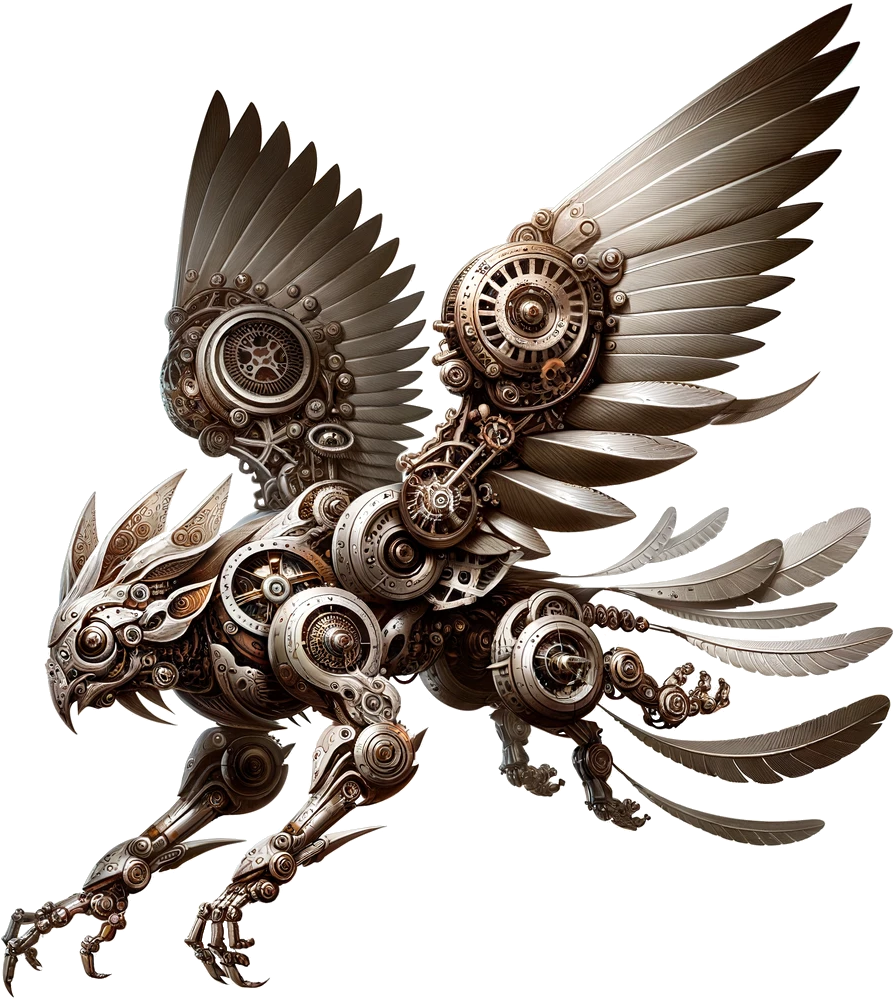
\includegraphics[width=0.175\paperwidth, keepaspectratio]{images/Homunculus_Servant.png}};
%\end{tikzpicture}
%\eject
%The homunculus is friendly to you and your companions, and it obeys your commands. See this creature's game statistics in the Homunculus Servant stat block, which uses your proficiency bonus (PB) in several places.
%
%In combat, the homunculus shares your initiative count, but it takes its turn immediately after yours. It can move and use its reaction on its own, but the only action it takes on its turn is the Dodge action, unless you take a bonus action on your turn to command it to take another action. That action can be one in its stat block or some other action. If you are incapacitated, the homunculus can take any action of its choice, not just Dodge.
%
%The homunculus regains 2d6 hit points if the mending spell is cast on it. If you or the homunculus dies, it vanishes, leaving its heart in its space.
%\paragraph*{Replicate Magic Item}\hfill\\
%\textbf{Taken: 1}\\
%Using this infusion, you replicate a particular magic item. You can learn this infusion multiple times; each time you do so, choose a magic item that you can make with it, picking from the Replicable Items tables. A table's title tells you the level you must be in the class to choose an item from the table. Alternatively, you can choose the magic item from among the common magic items in the game, not including potions or scrolls.
%
%In the tables, an item's entry tells you whether the item requires attunement. See the item's description in the Dungeon Master's Guide for more information about it, including the type of object required for its making.
%
%If you have Xanathar's Guide to Everything, you can choose from among the common magic items in that book when you pick a magic item you can replicate with this infusion.
%\subparagraph*{Rope of Climbing}
%This 60-foot length of silk rope weighs 3 pounds and can hold up to 3,000 pounds. If you hold one end of the rope and use an action to speak the command word, the rope animates. As a bonus action, you can command the other end to move toward a destination you choose. That end moves 10 feet on your turn when you first command it and 10 feet on each of your turns until reaching its destination, up to its maximum length away, or until you tell it to stop. You can also tell the rope to fasten itself securely to an object or to unfasten itself, to knot or unknot itself, or to coil itself for carrying.
%
%If you tell the rope to knot, large knots appear at 1-foot intervals along the rope. While knotted, the rope shortens to a 50-foot length and grants advantage on checks made to climb it.
%
%The rope has AC 20 and 20 hit points. It regains 1 hit point every 5 minutes as long as it has at least 1 hit point. If the rope drops to 0 hit points, it is destroyed.
%\subsubsection*{Infusing an Item}
%Whenever you finish a long rest, you can touch a nonmagical object and imbue it with one of your artificer infusions, turning it into a magic item. An infusion works on only certain kinds of objects, as specified in the infusion's description. If the item requires attunement, you can attune yourself to it the instant you infuse the item. If you decide to attune to the item later, you must do so using the normal process for attunement (see the attunement rules in the Dungeon Master's Guide).
%
%Your infusion remains in an item indefinitely, but when you die, the infusion vanishes after a number of days equal to your Intelligence modifier (minimum of 1 day). The infusion also vanishes if you replace your knowledge of the infusion.
%
%You can infuse more than one nonmagical object at the end of a long rest; the maximum number of objects appears in the Infused Items column of the Artificer table. You must touch each of the objects, and each of your infusions can be in only one object at a time. Moreover, no object can bear more than one of your infusions at a time. If you try to exceed your maximum number of infusions, the oldest infusion ends, and then the new infusion applies.
%
%If an infusion ends on an item that contains other things, like a bag of holding, its contents harmlessly appear in and around its space.
%\subsection*{Artificer Specialist (Battle Smith)}
%Armies require protection, and someone has to put things back together if defenses fail. A combination of protector and medic, a Battle Smith is an expert at defending others and repairing both materiel and personnel. To aid in their work, Battle Smiths are accompanied by a steel defender, a protective companion of their own creation. Many soldiers tell stories of nearly dying before being saved by a Battle Smith and a steel defender.
%
%In the world of Eberron, Battle Smiths played a key role in House Cannith's work on battle constructs and the original warforged, and after the Last War, these artificers led efforts to aid those who were injured in the war's horrific battles.
%\subsubsection*{Battle Smith Spells}
%Starting at 3rd level, you always have certain spells prepared after you reach particular levels in this class, as shown in the Battle Smith Spells table. These spells count as artificer spells for you, but they don't count against the number of artificer spells you prepare.
%\begin{DndTable}[header=Battle Smith Spells]{llX}
%			& \textbf{Artificer Level}  &\textbf{Battle Smith Spells}		\\
%$\bullet$	& 3rd						&Heroism, Shield					\\
%			& 5th						&Branding Smite, Warding Bond		\\
%			& 9th						&Aura of Vitality, Conjure Barrage	\\
%			& 13th						&Aura of Purity, Fire Shield		\\
%			& 17th						&Banishing Smite, Mass Cure Wounds	\\
%\end{DndTable}
%\subsubsection*{Battle Ready}
%When you reach 3rd level, your combat training and your experiments with magic have paid off in two ways:
%\begin{itemize}
%	\item You gain proficiency with martial weapons.
%	\item When you attack with a magic weapon, you can use your Intelligence modifier, instead of Strength or Dexterity modifier, for the attack and damage rolls.
%\end{itemize}
%\subsubsection*{Steel Defender}
%By 3rd level, your tinkering has borne you a faithful companion, a steel defender. It's friendly to you and your companions, and it obeys your commands. See its game statistics in the Steel Defender stat block, which uses your proficiency bonus (PB) in several places. You determine the creature's appearance and whether it has two legs or four; your choice has no effect on its game statistics.
%
%In combat, the defender shares your initiative count, but it takes its turn immediately after yours. It can move and use its reaction on its own, but the only action it takes on its turn is the Dodge action, unless you take a bonus action on your turn to command it to take another action. That action can be one in its stat block or some other action. If you are incapacitated, the defender can take any action of its choice, not just Dodge.
%
%If the Mending spell is cast on it, it regains 2d6 hit points. If it has died within the last hour, you can use your smith's tools as an action to revive it, provided you are within 5 feet of it and you expend a spell slot of 1st level or higher. The steel defender returns to life after 1 minute with all its hit points restored.
%
%At the end of a long rest, you can create a new steel defender if you have smith's tools with you. If you already have a defender from this feature, the first one immediately perishes. The defender also perishes if you die.
%\begin{DndMonster}[width=0.5\textwidth]{Steel Defender}
%    \DndMonsterType{Medium Construct}
%
%    % If you want to use commas in the key values, enclose the values in braces.
%    \DndMonsterBasics[
%        armor-class = {15 (Natural Armor)},
%        hit-points  = {\intcalcAdd{2}{\intcalcAdd{\calculateModifier{\IntelligenceScoreValue}}{\intcalcMul{5}{\LevelValue}}} (\LevelValue d8)},
%        speed       = {40 ft.},
%    ]
%    
%	\renewcommand{\AbilityScoreSpacer}{~}
%    \DndMonsterAbilityScores[
%		str = 14,
%		dex = 12,
%		con = 14,
%		int = 4,
%		wis = 10,
%		cha = 6,
%    ]
%
%    \DndMonsterDetails[
%        saving-throws = {Dex +\intcalcAdd{1}{\ProficiencyValue}, Con +\intcalcAdd{2}{\ProficiencyValue}},
%        skills = {Athletics +\intcalcAdd{2}{\ProficiencyValue}, Perception +\intcalcAdd{0}{\intcalcMul{2}{\ProficiencyValue}}},
%        %damage-vulnerabilities = {cold},
%        %damage-resistances = {bludgeoning, piercing, and slashing from nonmagical attacks},
%        damage-immunities = {poison},
%        senses = {Darkvision 60 ft., Passive Perception \intcalcAdd{10}{\intcalcMul{2}{\ProficiencyValue}}},
%        condition-immunities = {charmed, exhaustion, poisoned},
%        languages = {understands the languages you speak},
%        challenge = 1,
%    ]
%    
%    \DndMonsterAction{Vigilant}
%    The defender can't be surprised.
%	
%	\DndMonsterSection{Actions}	
%	\DndMonsterAttack[
%      name=Force-Empowered Rend,
%      distance=melee, % valid options are in the set {both,melee,ranged},
%      %type=weapon, %valid options are in the set {weapon,spell}
%      mod=\calculateSpellAttack{\calculateModifier{\IntelligenceScoreValue}},
%      reach=5,
%      %range=30,
%      targets=one target you can see,
%      dmg=1d8 + \intcalcAdd{0}{\ProficiencyValue},
%      dmg-type=force,
%      %plus-dmg=,
%      %plus-dmg-type=,
%      %or-dmg=,
%      %or-dmg-when=,
%      %extra=,
%    ]
%    
%    \DndMonsterAction{Repair (3/Day)}
%    The magical mechanisms inside the defender restore 2d8 + \intcalcAdd{0}{\ProficiencyValue} hit points to itself or to one construct or object within 5 feet of it.
%    
%    \DndMonsterSection{Reactions}
%    \DndMonsterAction{Deflect Attack}
%    The defender imposes disadvantage on the attack roll of one creature it can see that is within 5 feet of it, provided the attack roll is against a creature other than the defender.
%\end{DndMonster}
%\begin{tikzpicture}[remember picture, overlay]
%	\node[opacity=1,inner sep=0pt, xshift=-3cm, yshift=-2.25cm] at (current page.north east){
\includegraphics[width=0.175\paperwidth, keepaspectratio]{images/Steel_Defender.png}};
%\end{tikzpicture}
%\vspace*{-2.4\fontdimen6\font}\hfill\\
%\subsection*{The Right Tool for the Job}
%At 3rd level, you've learned how to produce exactly the tool you need: with thieves' tools or artisan's tools in hand, you can magically create one set of artisan's tools in an unoccupied space within 5 feet of you. This creation requires 1 hour of uninterrupted work, which can coincide with a short or long rest. Though the product of magic, the tools are nonmagical, and they vanish when you use this feature again.

\vfill\eject
\section*{Spells}
\textbf{Number of Leveled Spells (without Features):} \intcalcAdd{\calculateModifier{\IntelligenceScoreValue}}{\intcalcMax{1}{\intcalcShr{\LevelValue}}}
\subsection*{Cantrips}

\DndSpellHeader
  {Mending}
  {Transmutation Cantrip}
  {1 Minute}
  {Touch}
  {V, S, M (two lodestones)}
  {Instantaneous}

This spell repairs a single break or tear in an object you touch, such as a broken chain link, two halves of a broken key, a torn cloak, or a leaking wineskin. As long as the break or tear is no larger than 1 foot in any dimension, you mend it, leaving no trace of the former damage.

This spell can physically repair a magic item or construct, but the spell can't restore magic to such an object.

\DndSpellHeader
  {Sword Burst}
  {Conjuration Cantrip}
  {1 Action}
  {Self (5-foot Radius)}
  {V}
  {Instantaneous}

You create a momentary circle of spectral blades that sweep around you. All other creatures within 5 feet of you must succeed on a Dexterity saving throw or take 1d6 force damage.

\subparagraph*{At Higher Levels} This spell's damage increases by 1d6 when you reach 5th level (2d6), 11th level (3d6), and 17th level (4d6).

\subsection*{Level 1}

\DndSpellHeader
  {Absorb Elements}
  {1st-Level Abjuration}
  {1 Reaction, which you take when you take Acid, Cold, Fire, Lightning, or Thunder Damage}
  {Self}
  {S}
  {1 Round}

The spell captures some of the incoming energy, lessening its effect on you and storing it for your next melee attack. You have resistance to the triggering damage type until the start of your next turn. Also, the first time you hit with a melee attack on your next turn, the target takes an extra 1d6 damage of the triggering type, and the spell ends.

\subparagraph*{At Higher Levels} When you cast this spell using a spell slot of 2nd level or higher, the extra damage increases by 1d6 for each slot level above 1st.

\DndSpellHeader
  {Arcane Weapon}
  {1st-Level Transmutation}
  {1 Bonus Action}
  {Self}
  {V, S}
  {Concentration, Up to 1 Hour}

You channel arcane energy into one simple or martial weapon you're holding, and choose one damage type: acid, cold, fire, lightning, poison, or thunder. Until the spell ends, you deal an extra 1d6 damage of the chosen type to any target you hit with the weapon. If the weapon isn't magical, it becomes a magic weapon for the spell's duration.

As a bonus action, you can change the damage type, choosing from the options above.

\subparagraph*{At Higher Levels} When you cast this spell using a spell slot of 3rd level or higher, you can maintain your concentration on the spell for up to 8 hours.

\DndSpellHeader
  {Faerie Fire}
  {1st-Level Evocation}
  {1 Action}
  {60 feet}
  {V}
  {Concentration, Up to 1 Minute}

Each object in a 20-foot cube within range is outlined in blue, green, or violet light (your choice).

Any creature in the area when the spell is cast is also outlined in light if it fails a Dexterity saving throw. For the duration, objects and affected creatures shed dim light in a 10-foot radius.

Any attack roll against an affected creature or object has advantage if the attacker can see it, and the affected creature or object can't benefit from being invisible.

%\DndSpellHeader
%  {Heroism}
%  {1st-Level Enchantment}
%  {1 Action}
%  {Touch}
%  {V, S)}
%  {Concentration, Up to 1 Minute}
%
%A willing creature you touch is imbued with bravery. Until the spell ends, the creature is immune to being frightened and gains temporary hit points equal to your spellcasting ability modifier at the start of each of its turns. When the spell ends, the target loses any remaining temporary hit points from this spell.
%
%\subparagraph*{At Higher Levels} When you cast this spell using a spell slot of 2nd level or higher, you can target one additional creature for each slot level above 1st.
%
%\DndSpellHeader
%  {Shield}
%  {1st-Level Abjuration}
%  {1 Reaction, which you take when you are hit by an attack or targeted by the Magic Missile spell}
%  {Self}
%  {V, S)}
%  {1 Round}
%
%An invisible barrier of magical force appears and protects you. Until the start of your next turn, you have a +5 bonus to AC, including against the triggering attack, and you take no damage from magic missile.

\DndSpellHeader
  {Tasha's Caustic Brew}
  {1st-Level Evocation}
  {1 Action}
  {Self (30-foot line)}
  {V, S, M (a bit of rotten food)}
  {Concentration, Up to 1 Minute}

A stream of acid emanates from you in a line 30 feet long and 5 feet wide in a direction you choose. Each creature in the line must succeed on a Dexterity saving throw or be covered in acid for the spell's duration or until a creature uses its action to scrape or wash the acid off itself or another creature. A creature covered in the acid takes 2d4 acid damage at start of each of its turns.

\subparagraph*{At Higher Levels} When you cast this spell using a spell slot 2nd level or higher, the damage increases by 2d4 for each slot level above 1st.

\vfill\eject
\section*{Miscellaneous}
\subsection*{Attack and Damage Rolls}
\subsubsection*{Melee Weapons}
\paragraph*{Attack Roll}\hfill\\
\underline{\textit{Lance (Special):}}\\
1d20 + STR-Modifier + Proficiency Modifier\\
\indent Current Max: \intcalcAdd{20}{\intcalcAdd{\calculateModifier{\StrengthScoreValue}}{\ProficiencyValue}}
\\
\underline{\textit{Handaxe (Throwable):}}\\
1d20 + STR-Modifier + Proficiency Modifier\\
\indent Current Max (melee): \intcalcAdd{20}{\intcalcAdd{\calculateModifier{\StrengthScoreValue}}{\ProficiencyValue}}\\
\indent Current Max (thrown): \intcalcAdd{20}{\intcalcAdd{\calculateModifier{\StrengthScoreValue}}{\ProficiencyValue}}
\\
\underline{\textit{Quarterstaff (Versatile):}}\\
1d20 + STR-Modifier + Proficiency Modifier\\
\indent Current Max: \intcalcAdd{20}{\intcalcAdd{\calculateModifier{\StrengthScoreValue}}{\ProficiencyValue}}
\\
\underline{\textit{Magic Weapon:}}\\
1d20 + INT-Modifier + Proficiency Modifier\\
\indent Current Max: \intcalcAdd{20}{\intcalcAdd{\calculateModifier{\IntelligenceScoreValue}}{\ProficiencyValue}}
\paragraph*{Damage Roll}\hfill\\
\underline{\textit{Lance (Special):}}\\
1d12 + STR-Modifier\\
\indent Current Max: \intcalcAdd{12}{\calculateModifier{\StrengthScoreValue}}
\\
\underline{\textit{Handaxe (Throwable):}}\\
1d6 + STR-Modifier\\
\indent Current Max (melee): \intcalcAdd{6}{\calculateModifier{\StrengthScoreValue}}\\
\indent Current Max (thrown): \intcalcAdd{6}{\calculateModifier{\StrengthScoreValue}}
\\
\underline{\textit{Quarterstaff (Versatile):}}\\
1d6 (1d8) + STR-Modifier\\
\indent Current Max (one-handed): \intcalcAdd{6}{\calculateModifier{\StrengthScoreValue}}\\
\indent Current Max (two-handed): \intcalcAdd{8}{\calculateModifier{\StrengthScoreValue}}
\\
\underline{\textit{Magic Weapon Damage Bonus:}}\\
INT-Modifier\\
\indent Bonus: \calculateModifier{\IntelligenceScoreValue}
\subsubsection*{Ranged Weapons}
\paragraph*{Attack Roll}\hfill\\
\underline{\textit{Light Crossbow:}}\\
1d20 + DEX-Modifier + Proficiency Modifier\\
\indent Current Max: \intcalcAdd{20}{\intcalcAdd{\calculateModifier{\DexterityScoreValue}}{\ProficiencyValue}}
\paragraph*{Damage Roll}\hfill\\
\underline{\textit{Light Crossbow:}}\\
1d6 + DEX-Modifier\\
\indent Current Max: \intcalcAdd{6}{\calculateModifier{\DexterityScoreValue}}
\subsubsection*{Special Attacks}
\paragraph*{Attack Roll}\hfill\\
\underline{\textit{Unarmed Strike:}}\\
1d20 + STR-Modifier + Proficiency Modifier\\
\indent Current Max: \intcalcAdd{20}{\intcalcAdd{\calculateModifier{\StrengthScoreValue}}{\ProficiencyValue}}
\paragraph*{Damage Roll}\hfill\\
\underline{\textit{Unarmed Strike:}}\\
1 + STR-Modifier\\
\indent Current Max: \intcalcAdd{1}{\calculateModifier{\StrengthScoreValue}}
\end{document}
